\chapter{Doppler Layer}

\section{Introduction}
In this section we will explore the implementation of a new plugin in the ROS navigation stack based on the radar's relative radial velocity information. The plugin proposed is a map layer and can be specified by either the global or local costmap. The objective of said layer is to increase the cost values of cells based on the prediction of the motion of said obstacles provided by the radar (doppler channel). The ending result should be a better avoidance of incoming obstacles with negative relative velocity  to the robot.

\section{Layered Costmaps}
As said before the global and local costmaps used in \ac{ROS} Navigation Stack are both layered costmaps.
This means that they are composed by independent components with each one affecting the resulting layered costmap in specific environmental contexts. For example the classic \textit{static layer} takes information from a published map topic and based on the position of the robot marks some  pre-determined obstacles.  Figure \ref{fig::layers} show some different layers for different contexts.
\begin{figure}[h] 
\centerline{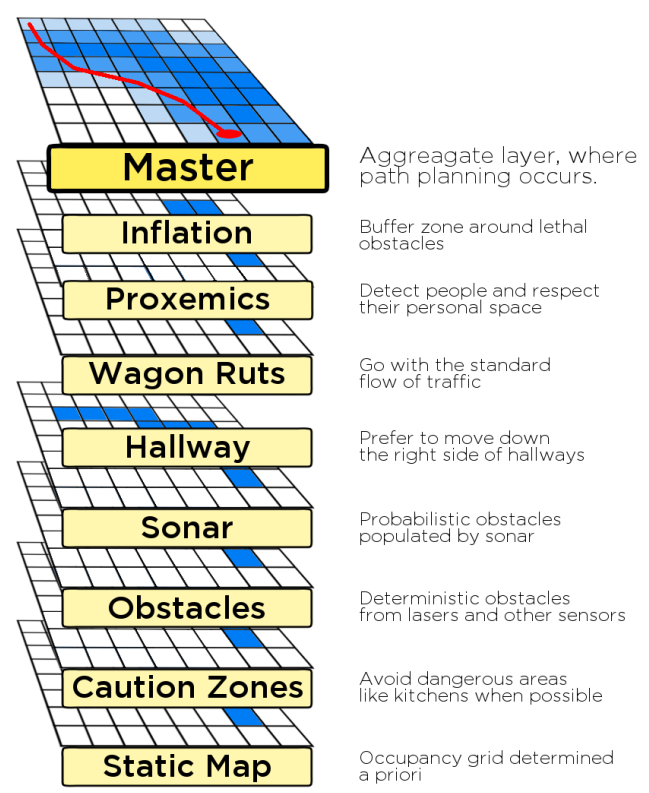
\includegraphics [width=0.5 \textwidth]{imgs/chapter6/layers.png}}
\caption{A stack of costmap layers, showcasing the different contextual
behaviors achievable with the layered costmap approach from \cite{lu2014layered}}
\label{fig::layers}
\end{figure}

The set of layers used follows a specific hierarchy that determines what order and how they overwrite the master costmap. This is an important part to take into consideration the priority


\section{Field Testing}

%\subsection{Side Tracking}

%\subsection{Target Speed Limitations}

%\section{Summary}